\subsection{Wasser}

\subsubsection{Schweiz}
Die Schweiz wird oft als das Wasserschloss von Europa bezeichnet. «Viele wichtige Flüsse Europas – Rhein, Rhone, Inn (Donau) und Tessin (Po), Etsch (Adige) – nehmen ihren Ursprung hierzulande. Obschon die Schweiz flächenmässig nur knapp vier Promille am Kontinent ausmacht, befinden sich auf ihrem Boden sechs Prozent der Süsswasservorräte Europas». („Wasserschloss Schweiz - NZZ“, o. J.)
\begin{figure}[H]
	\centering
	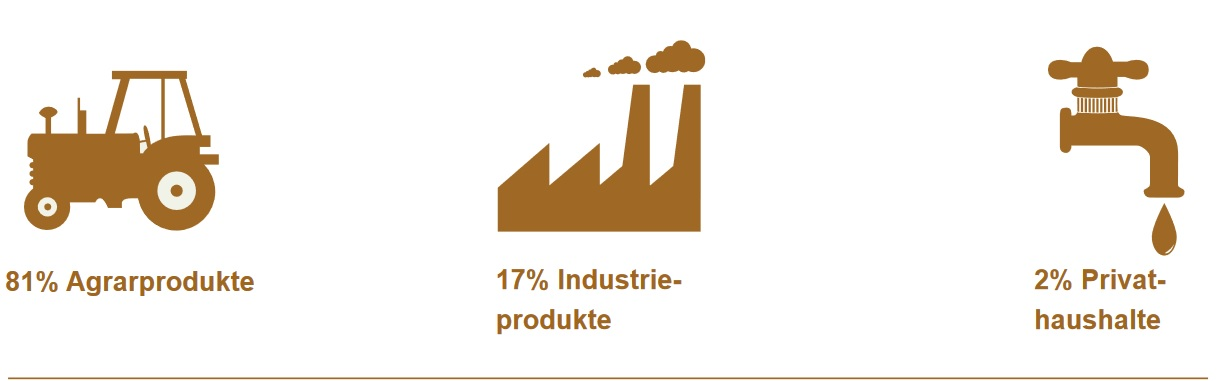
\includegraphics[width=0.9\textwidth]{WV}
	\caption{Wasserverbrauch aufgeteilt nach Sektoren}
\end{figure}
Der Gesamtwasserverbrauch in der Schweiz liegt bei 1960 Mio. $m^3/Jahr$ dieser Verbrauch teilt sich auf auf die Privathaushalte (2\%), Industrie (17\%) und auf den Agrarsektor (83\%) auf. Die Wein und Bierproduktion braucht hierzulande nur 3\% des Agrarwasserverbrauchs. Für die Weinproduktion muss in der Schweiz nur sehr wenig Wasser eingesetzt werden, da die Niederschläge meistens ausreichen. (Wettstein u. a., 2016)
\begin{figure}[H]
	\centering
	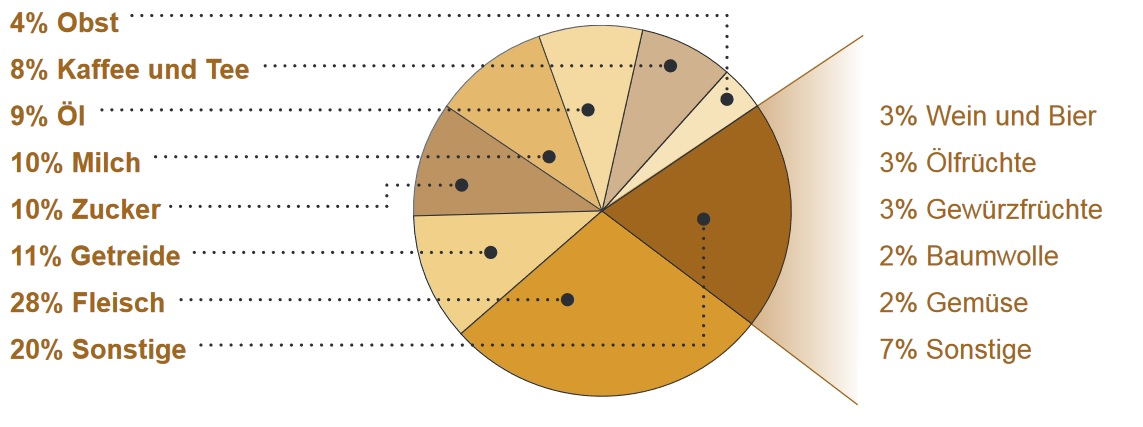
\includegraphics[width=0.9\textwidth]{WVA}
	\caption{Anteile des Wasserverbrauchs im       Agrarsektor}
\end{figure}

Durch die grosse Verfügbarkeit und die geringe Nutzung von Wasser für den Weinbau ist der Wasserverbrauch für Wein in der Schweiz nicht problematisch. Jedoch sind die Wasserverschmutzungen die durch die Weinproduktion entstehen nicht unproblematisch. Zur Wasserverschmutzung tragen vor allem Ausschwemmungen von Pestiziden bei.

\subsubsection{Kalifornien}
\label{sub:wasserverbrauch}

In Kalifornien werden etwa 42'000 $m^3$ Wasser für die Landwirtschaft benötigt. Das entspricht  39 \% des gesamten
Wasserverbrauchs. 

Der Wasserverbrauch beim Weinanbau ist grundsätzlich nicht so hoch wie bei anderen Pflanzen. Es
werden dennoch rund 700 Liter Wasser pro Liter Wein benötigt.
(\glqq{}The Water Footprint of the Wine Industry\grqq{} (2015)). 

In Kalifornien
herrscht seit 2011 eine Dürre, die Wasserrationierung nötig machte. Daher regulieren über 90 \% der
Weingüter aktiv ihre Bewässerung. Die grösste Einsparung gibt es durch die Tropfbewässerung. Dabei
wird das Wasser direkt den Wurzeln  des Weinstocks zugefügt. Dabei verdunstet weniger Wasser
unbenutzt.

Zusätzlich fliesst auch kein Wasser ab und es werden keine Nährstoffe ausgeschwemmt. Das reduziert
den Einsatz von Dünger und die Eutrophierung des Grundwassers.

Wo es der Untergrund zulässt, wird auf Trockenfeldbau gesetzt.

(\glqq{}California Wine Community Sustainability Report Appendix\grqq{} (2015)).


Auch bei der Produktion in den Kellereien wurde Massnahmen getroffen, um das verwendete Wasser zu
reduzieren. Hier fällt es vor allem für die Reinigung der Gärtanks an. Dieses Wasser wird nun
aufgefangen und wiederverwendet.
